\begin{table}[htbp]\centering
\begin{tabular}{lrr}\toprule
Outcome & Work exposure & Matched control\\\midrule
Direct interpretation & 12/12 & 0/12 \\
Nested composition & 12/12 & 0/12 \\
Total correct answers & 24/24 & 0/24 \\
Valid response objects & 12/12 & 12/12 \\
\bottomrule\end{tabular}
\caption{Observed pilot results. Answers within one context are clustered; the primary analysis has 12 domain pairs.}
\label{tab:pilot}
\end{table}
All 12 paired domain differences were +1 on the mean-correctness scale, so the observed paired mean gain was $\widehat G=1.0$. Every control response was $(5,5)$; none of the pre-generated answer keys was 5. The generated dataset was fixed before any response, with no dataset selection based on outcomes.

The predeclared paired-label test enumerated all $2^{12}=4096$ assignments. Its directional null-tail probability was $1/4096=0.000244140625$, and its two-sided probability was $2/4096=0.00048828125$. The exact sign test agreed. These results require the stated paired exchangeability and domain-level independence assumptions.

\begin{figure}[htbp]\centering
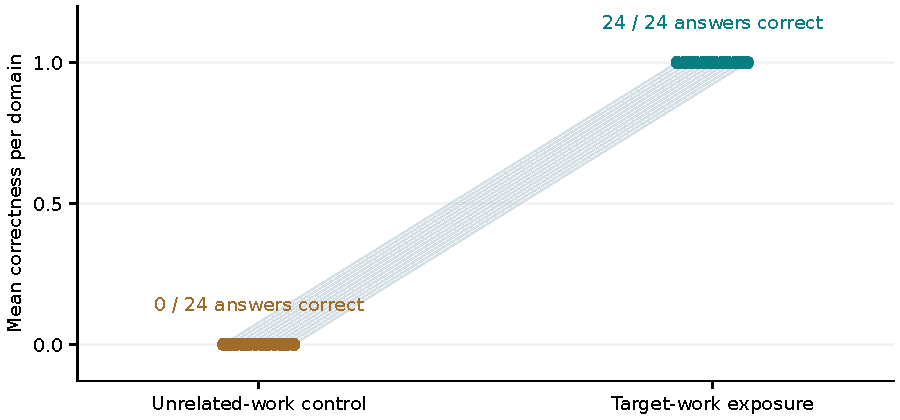
\includegraphics[width=0.85\linewidth]{figures/pilot.pdf}
\caption{Observed encounter-time pilot. Each mark is one domain-paired mean score, based on two answers in one fresh context per condition. There are 12 instances of one generated function class. No per-query output-distribution or training-support estimate is plotted.}
\label{fig:pilot}
\end{figure}
\textbf{Exploratory bound.} Separately from the predeclared tests, Equation~\eqref{eq:gainci} with $\alpha=0.05$ gives $G\ge 0.2934$ and hence $I\ge 0.2934$ for the same fixed 12-domain benchmark, conditional on independent response pairs and a stable interface. At an illustrative threshold $\epsilon=0.10$, Equation~\eqref{eq:meanbounds} gives $\AIP_{0.10}\ge 0.2149$ on that same coverage event. This is a conservative one-sided 95\% bound under those assumptions, not a point estimate or a coefficient fitted to the pooling law. The backend's independence and checkpoint stability were not directly observable.
